\documentclass[t,aspectratio=169]{beamer}
%\usetheme{Berkeley}
\usepackage{graphicx}
\usepackage{amsmath}
\usepackage[american]{circuitikz}

\title{Clase 26}
\subtitle{Modelo de CA del transistor MOSFET}
\author{Dr.-Ing. Juan José Montero Rodríguez}
\subject{Elementos Activos}
\institute{Escuela de Ingeniería Electrónica}
\date{Semestre II-2023}
\titlegraphic{
\includegraphics[height=8mm]{./figuras/logotec.pdf}}

\begin{document}

\begin{frame}{}
\maketitle
\end{frame}


\section{Transconductancia}
\begin{frame}{Transconductancia}

\begin{columns}

\begin{column}{0.5\textwidth}

    La transconductancia es una medida de la capacidad de un transistor para convertir una tensión de entrada a corriente de salida.

    \vspace{5mm}
    La transconductancia de un MOSFET se define como: 
    %
    \[ g_m = \dfrac{\partial I_D}{\partial V_{GS}} \]
    %
    es decir, g\textsubscript{m} es la pendiente de la curva característica de transferencia en el punto de operación
     
\end{column}

\begin{column}{0.5\textwidth}

	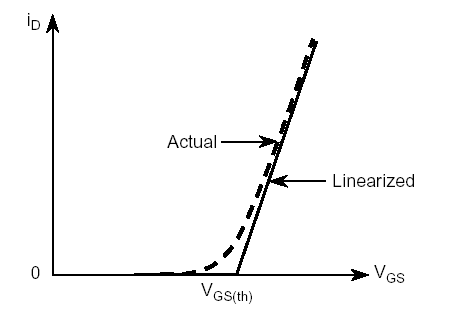
\includegraphics[width=6.5cm]{./figuras/transcond.png}
 
\end{column}

\end{columns}


\end{frame}


\begin{frame}{Transconductancia}

Aplicando la definición:
%
\[ g_m =  \dfrac{d}{dV_{GS}} \left\{ \dfrac{1}{2} \mu_n C_{ox}' \dfrac{W}{L} (V_{GS} - V_{TH})^2 \right\} \]
%
\[ \boxed{g_m =  \mu_n C_{ox}' \dfrac{W}{L} (V_{GS} - V_{TH})} \]

Otra forma de expresar la transconductancia se obtiene dividiendo $g_m$ entre $I_D$:
%
\[ \dfrac{g_m}{I_D} = \dfrac{\mu_n C_{ox}' \dfrac{W}{L} (V_{GS} - V_{TH})}{\dfrac{1}{2} \mu_n C_{ox}' \dfrac{W}{L} (V_{GS} - V_{TH})^2} \Rightarrow \boxed{g_m = \dfrac{2I_D}{V_{GS} - V_{TH}}} \]
    
\end{frame}


\begin{frame}{Transconductancia}

\begin{columns}

\begin{column}{0.5\textwidth}

Una tercera forma de expresar la transconductancia se obtiene partiendo de la primera:
\[ g_m =  \mu_n C_{ox}' \dfrac{W}{L} (V_{GS} - V_{TH}) \]

Despejando $V_{GS} - V_{TH}$:
\[ (V_{GS} - V_{TH}) = \dfrac{g_m}{\mu_n C_{ox}' \dfrac{W}{L}} \]

Y sustituyendo en la ecuación de $I_D$:
\[ I_D = \dfrac{1}{2} \mu_n C_{ox}' \dfrac{W}{L} (V_{GS} - V_{TH})^2 \]

\end{column}

\begin{column}{0.5\textwidth}

Se obtiene lo siguiente:
\[ I_D = \dfrac{1}{2} \mu_n C_{ox}' \dfrac{W}{L} \left(\dfrac{g_m}{\mu_n C_{ox}' \dfrac{W}{L}}\right)^2 \]

Despejando la transconductancia:
\[ \boxed{g_m = \sqrt{2 \mu_n C_{ox}' \dfrac{W}{L} I_D}} \]

Las tres ecuaciones de transconductancia son válidas y deben dar el mismo valor.

\end{column}

\end{columns}

\end{frame}

\section{Modelo CA}
\begin{frame}{Modelo de pequeña señal}

\begin{figure}[H]
    \centering
    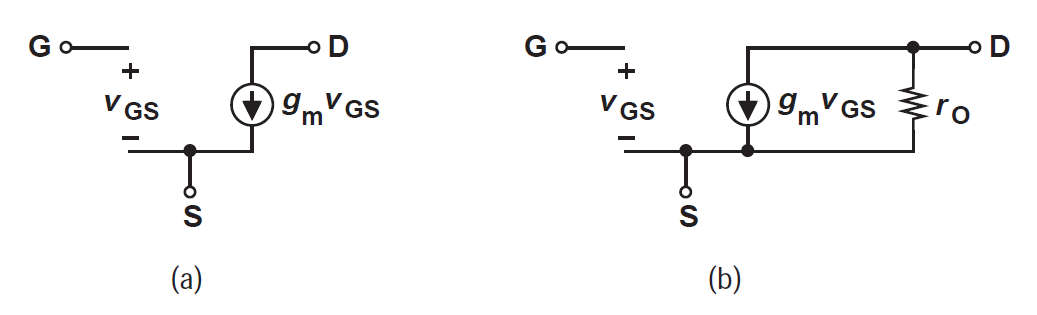
\includegraphics[width=0.8\textwidth]{figuras/modelo_ca_mosfet.png}
\end{figure}

La resistencia de salida se define como la pendiente de la curva de salida:
\[ r_o = \left( \dfrac{\partial I_D}{\partial V_{DS}} \right)^{-1} = \dfrac{1}{\dfrac{1}{2}\mu_n C_{ox}' \dfrac{W}{L} (V_{GS}-V_{TH})^2 \lambda} \Rightarrow \boxed{r_o = \dfrac{1}{\lambda I_D}} \]


\end{frame}


\begin{frame}{Procedimiento de solución de circuitos en CA}
Los pasos a seguir para obtener el equivalente de pequeña señal son:

\vspace{5mm}
\textbf{Modelo de gran señal}

\begin{itemize}
    \item Apagar las fuentes de CA, conectar las fuentes de CD.
    \item Reemplazar los condensadores por circuitos abiertos ($X_C = 1/j\omega{}C = \infty$).
    \item Determinar el punto de operación en CD, con las fuentes de CA apagadas.
\end{itemize}

\vspace{5mm}
\textbf{Modelo de pequeña señal}

\begin{itemize}
    \item Apagar las fuentes de CD, conectar las fuentes de CA.
    \item Reemplazar los condensadores por cortocircuitos ($X_C = 1/j\omega{}C \approx 0$).
    \item Calcular los parámetros de corriente alterna con los puntos de operación obtenidos.
    \item Reemplazar los elementos activos del circuito por sus equivalentes de pequeña señal de acuerdo con los parámetros de CA calculados.

\end{itemize}

\end{frame}




\section{Ejemplo 1}
\begin{frame}{Ejemplo 1: Solución de circuitos por superposición}

\begin{figure}[H]
    \centering
    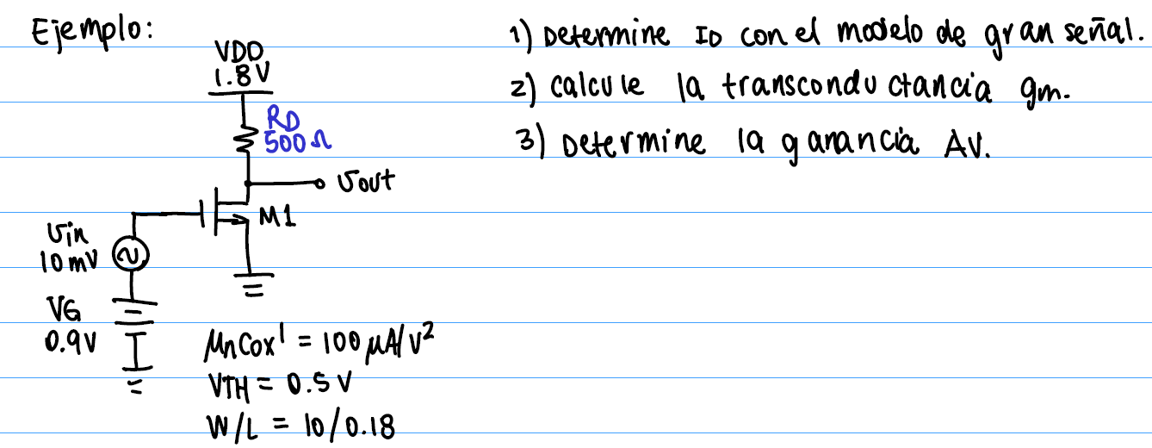
\includegraphics[width=\textwidth]{figuras/ejemplo_1_1.png}
\end{figure}

\end{frame}


\begin{frame}{Solución 1: Solución de circuitos por superposición}

\begin{figure}[H]
    \centering
    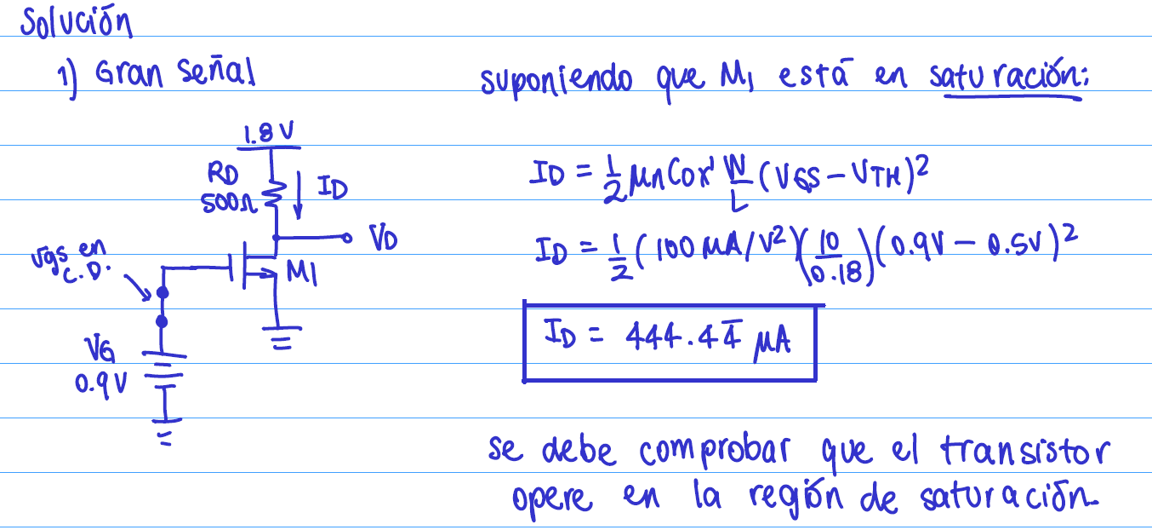
\includegraphics[width=\textwidth]{figuras/ejemplo_1_2.png}
\end{figure}

\end{frame}


\begin{frame}{Solución 1: Solución de circuitos por superposición}

\begin{figure}[H]
    \centering
    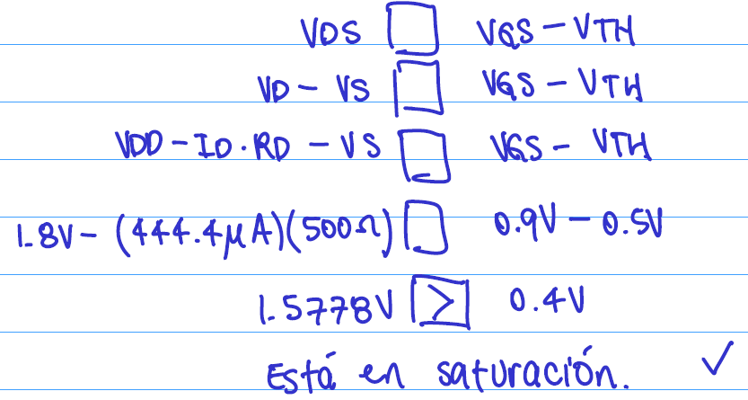
\includegraphics[width=0.6\textwidth]{figuras/ejemplo_1_3.png}
\end{figure}

\end{frame}


\begin{frame}{Solución 1: Solución de circuitos por superposición}
Otro método para calcular el punto de operación sin utilizar la cuadrática:

\begin{itemize}
    \item Las tres ecuaciones de transconductancia relacionan $I_D$, $V_{GS}$ y $W/L$.
    \item En este problema se conocen $V_{GS}$ y $W/L$.
    \item Se puede calcular $g_m$ y despejar luego $I_D$ con otra ecuación.
\end{itemize}

\begin{columns}

\begin{column}{0.5\textwidth}

La transconductancia es:
\begin{align*}
 g_m &= \mu_n C_{ox}' \dfrac{W}{L} (V_{GS} - V_{TH}) \\
 g_m &= (100\ \mu A/V^2) \dfrac{10}{0.18} (0.9\ V - 0.5\ V) \\
 g_m &= 2.22\ mS 
\end{align*}

\end{column}

\begin{column}{0.5\textwidth}

Con las otras ecuaciones de transconductancia:
\begin{align*}
g_m &= \dfrac{2I_D}{V_{GS} - V_{TH}} \\
I_D &= \dfrac{g_m(V_{GS} - V_{TH})}{2} \\
I_D &= \dfrac{(2.22\ mS)(0.9\ V-0.5\ V)}{2} \\
I_D &= 444.44\ \mu A
\end{align*}

\end{column}

\end{columns}

\end{frame}


\begin{frame}{Solución 1: Solución de circuitos por superposición}

\begin{figure}[H]
    \centering
    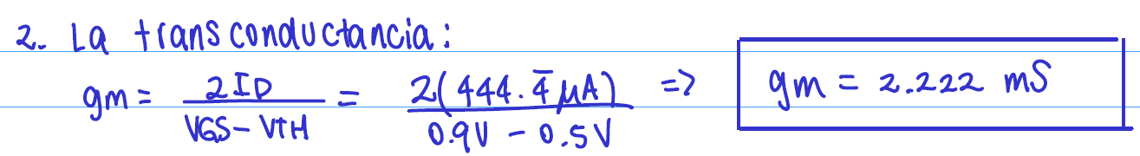
\includegraphics[width=\textwidth]{figuras/ejemplo_1_4.png}

    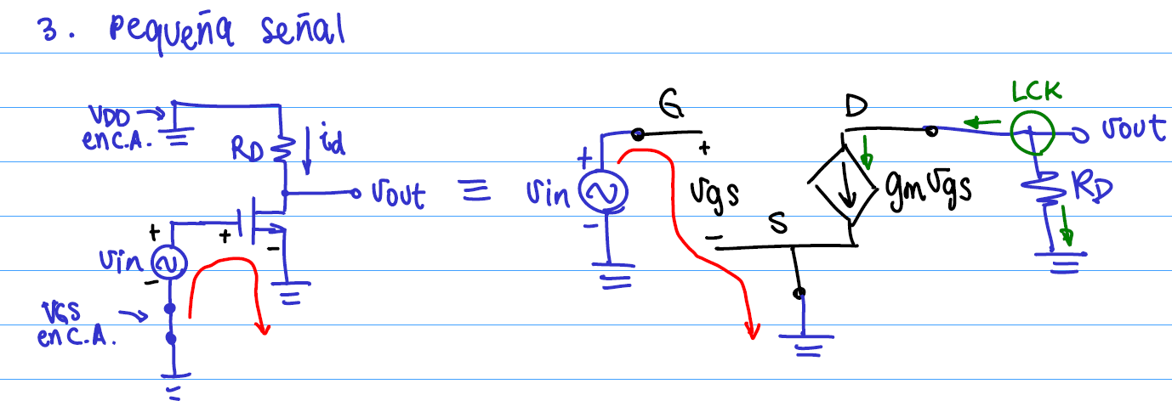
\includegraphics[width=\textwidth]{figuras/ejemplo_1_5.png}
\end{figure}

\end{frame}


\begin{frame}{Solución 1: Solución de circuitos por superposición}

\begin{figure}[H]
    \centering
    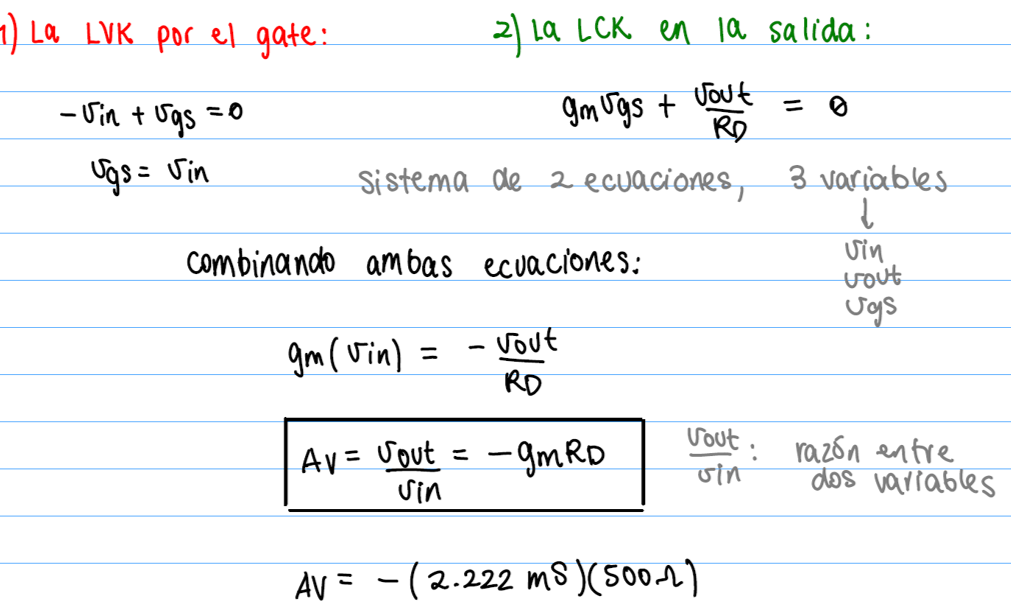
\includegraphics[width=0.8\textwidth]{figuras/ejemplo_1_6.png}
\end{figure}

\end{frame}


\begin{frame}{Solución 1: Solución de circuitos por superposición}

\begin{figure}[H]
    \centering
    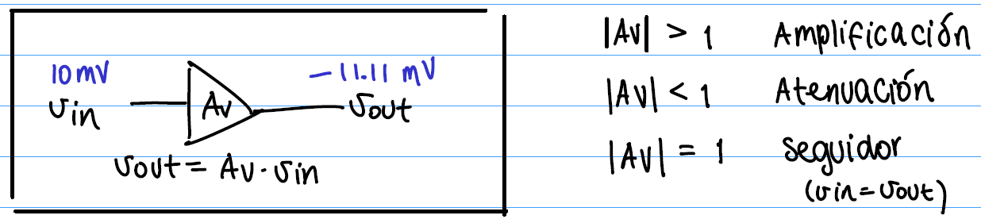
\includegraphics[width=0.8\textwidth]{figuras/ejemplo_1_7.png}

    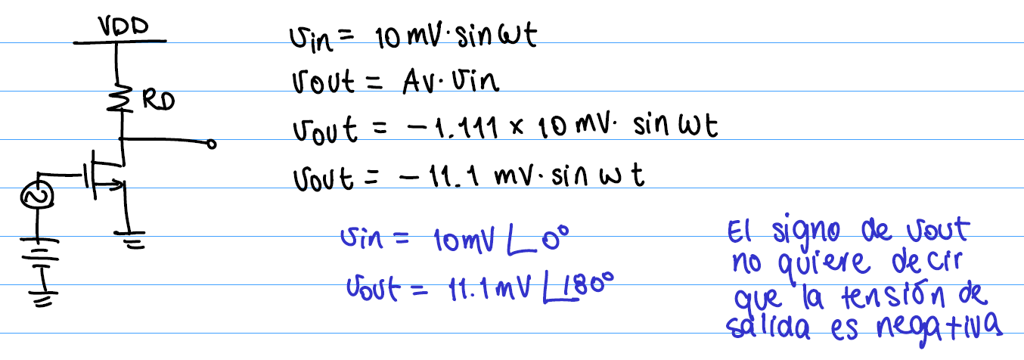
\includegraphics[width=0.8\textwidth]{figuras/ejemplo_1_8.png}
\end{figure}

\end{frame}


\section{Substrato}
\begin{frame}{Transconductancia de substrato}
La transconductancia de substrato de un MOSFET se define como:
%
\[ g_{mb} = \dfrac{\partial I_D}{\partial V_{BS}} \]
%
que también puede calcularse como
%
\[ g_{mb} = \chi g_m \]
%
Donde
%
\[ \chi = \dfrac{\partial V_{TH}}{\partial V_{SB}} = \dfrac{\gamma}{2\sqrt{2\phi_F+V_{SB}}} \]

Recordando que
\begin{itemize}
    \item $\gamma$: Coeficiente de efecto de substrato ($\sqrt{V}$).
    \item $\phi_F$: Diferencia entre nivel de Fermi y nivel intrínseco en oblea ($E_i - E_F$).
    \item $2\phi_F$: Potencial de superficie necesario para inversión ($\phi_S$).
\end{itemize}

\end{frame}



\begin{frame}{Modelo de pequeña señal en baja frecuencia}
En baja frecuencia, el modelo de pequeña señal del MOSFET es:

\begin{figure}
    \centering
    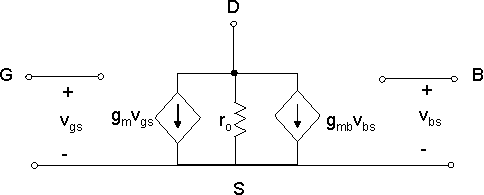
\includegraphics[width=11cm]{./figuras/peqsenal.pdf}
\end{figure}

Nótese que cuando $V_B < V_S$, el signo de $V_{bs}$ es negativo y la corriente de la fuente $g_{mb}V_{bs}$ cambia de dirección, indicando una reducción de la corriente entre drenador y surtidor, lo cual equivale a un aumento del voltaje de umbral
\end{frame}


\begin{frame}{Modelo de pequeña señal en alta frecuencia}
En alta frecuencia, el modelo de pequeña señal del MOSFET es:

\begin{figure}
    \centering
    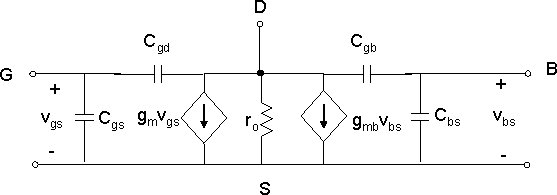
\includegraphics[width=11cm]{./figuras/peqsenal2.pdf}
\end{figure}

Los condensadores se encuentran en las interfaces P-N y en los óxidos laterales, que son puntos donde se acumula carga parásita (no deseada) y que limitan la frecuencia de operación máxima del transistor.

\end{frame}


\begin{frame}{Lecturas recomendadas}

\begin{itemize}
    \item Razavi, B. (2013). Fundamentals of microelectronics. Chapter 6: Physics of MOS transistors, 2nd ed., pp. 295-296, Wiley.
\end{itemize}

\end{frame}


\end{document}
